\subsection{Registration}
\begin{figure}
    \centering
    \begin{adjustbox}{width=\linewidth}
        \forestset{
          direction switch/.style={
            where level>=1{folder, grow'=0}{for children=forked edge},
          },
        }
        \begin{forest}
          direction switch
          [SR
            [MISR
              [Adapative Filtering]
              [Statistical
                [Back Projection]
                [Markov Random Fields]
                [Bilateral Total Variation]
              ]
            ]
            [SISR
                [Manifold Learning]
                [Compressed Sensing]
                [Projection]
                [Belief Networks]
            ]
          ]
        \end{forest}
    \end{adjustbox}
    \caption{Taxonomy of classical SR techniques}
    \label{fig:taxonomy}
\end{figure}

Figure~\ref{fig:taxonomy} lays out a rough taxonomy of classical SR algorithms.
%
We cover algorithms from each "genus" and others that don't neatly fit into the taxonomy.
\subsection{Interpolation}
Suppose that $H_k$ is linear spatial\anote{lsi} and time invariant.
%
Suppose further that $A_k$ is affine.
%
Then $H \coloneqq H_k$ commutes with $A_k$\cite{meladcommute} and equation~\ref{eqn:commuteimagingmodel} becomes
\begin{align}
    X_k &= (D_k \circ A_k \circ H) (Y) + \epsilon \\
    &= (D_k \circ A_k) (H(Y)) + \epsilon \\
    &= (D_k \circ A_k) (Z) + \epsilon
    \label{eqn:commuteimagingmodel}
\end{align}
This naturally suggests interpolation in order to recover $Z$ (since $X_k$, in this manifestation, is simply shifted samples of $Z$).
%
Note in this context we use interpolation very broadly, i.e. to connote filling in missing values using neighboring (in some sense --- not necessarily geometrically) values.
%
\begin{figure}
    \centering
    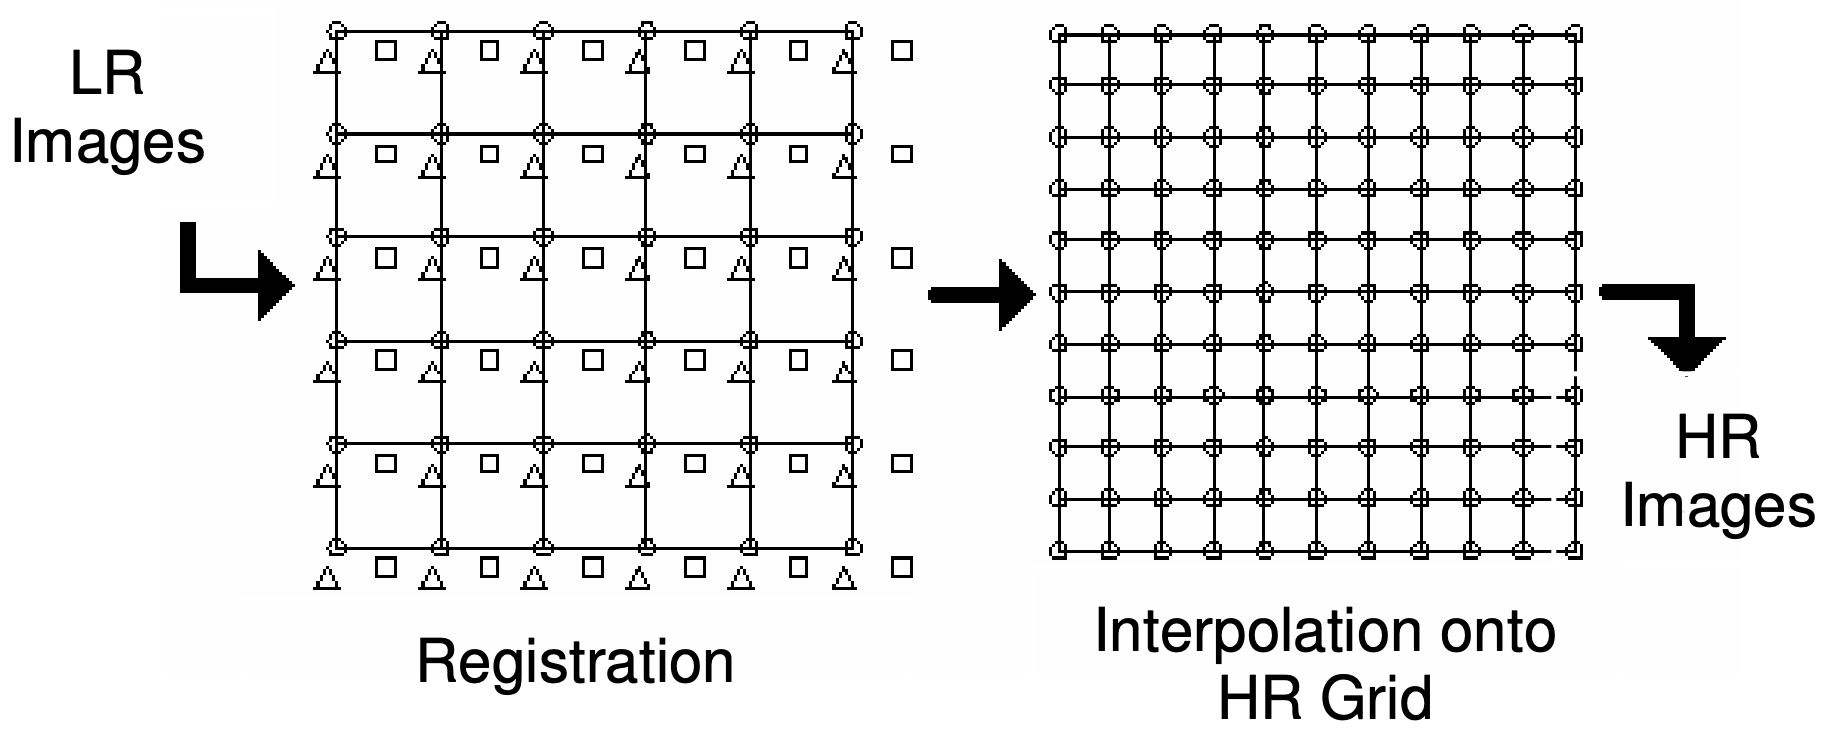
\includegraphics[width=\linewidth]{figures/hrgrid.png}
    \caption{LR image registration on an HR grid\cite{Lin}}
    \label{fig:hrgrid}
\end{figure}
This class of techniques proceed by first registering images on a high resolution grid (see figure~\ref{fig:hrgrid}) then interpolating at the "missing" pixels in the HR grid to recover $Z$, and finally denoising and deconvolution (of $H$) to recover $Y$.
%
Since in general consecutive $X_k$ have non-uniform shifts (relative to $X_0$) the interpolation is non-uniform and improvisations on this theme use various weighting schemes for the adjacent pixels.

For example Alam et. al\cite{Alam2000} uses weighted nearest neighbors: for every pixel to be interpolated the three nearest pixels are weighted inversely by their distance (according to HR grid distance) and then their weighted sum is assigned to that pixel.
%
This non-uniform interpolation is then followed by application of a Wiener filter whose design is informed by the OTF of the particular imaging system they study (which they do not estimate i.e. they assume they can model accurately).
%
\begin{figure}
    \centering
    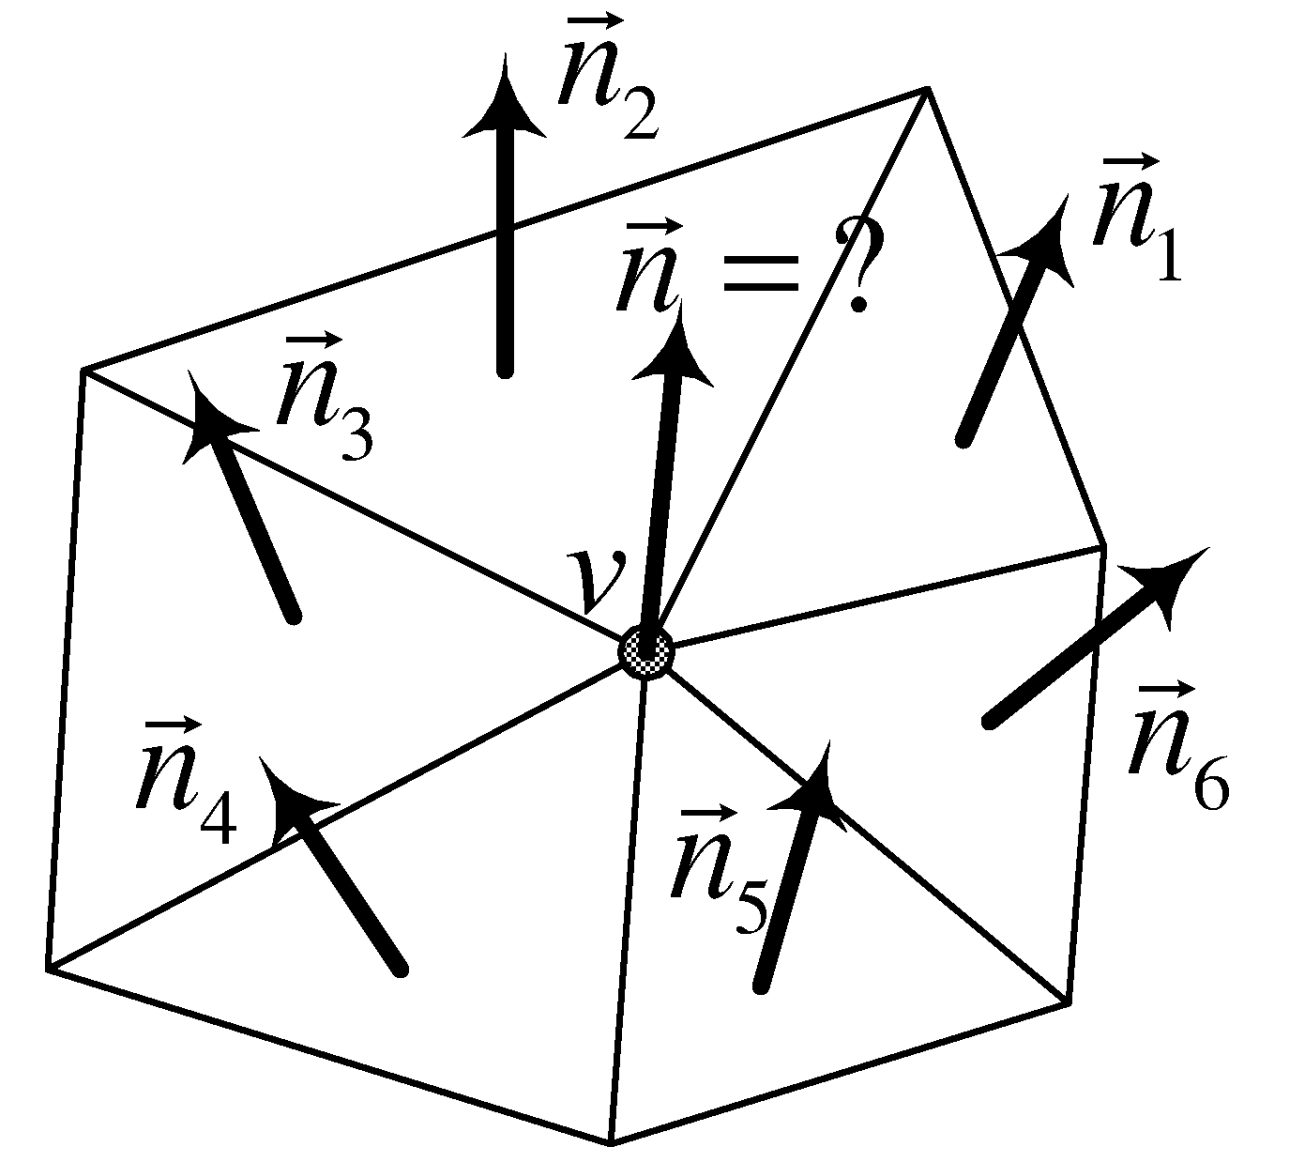
\includegraphics[width=.7\linewidth]{figures/delauney.png}
    \caption{Delaunay triangulation for fitting splines at LR pixels. $v$ is an LR pixel. Note that $v$ is at $z$ equal to the pixel value.}
    \label{fig:delauney}
\end{figure}
Lertrattanapanich et. al\cite{Lertrattanapanich} base their algorithm on interpolants which require knowledge of gradients (e.g. splines) and mediate the non-uniform sampling by using a weighted average (by area) of those gradients in adjacent Delaunay cells; to be precise they produce a Delaunay triangulation of all LR pixels\anote{lrpixel} and compute the gradients (see figure~\ref{fig:delauney}) according to
\begin{align*}
    \vec{n} = \sum_{j=1}^k \frac{A_j \vec{n_j}}{A} &\text{ where } A=\sum_{i=1}^k A_i\\
    \frac{\partial z}{\partial x} = -\frac{n_x}{n_z} &\text{ and }  \frac{\partial z}{\partial y} = -\frac{n_y}{n_z} \\
\end{align*}
Unfortunately this intricate solution is not robust to noise in real images.

A more sophisticated method for non-uniform interpolation uses parametric models for the auto-correlation between LR pixels and the cross-correlation between LR pixels and interpolated pixels to estimate wiener filter weights.
%
These weights are then used to average nearby pixel values.
%
The algorithm operates on a sliding window called the estimation window whose dimensions $D_x, D_y$ are chosen such that the effective sampling rate exceeds the Nyquist rate for a given $\rho_c$.
\begin{figure}
    \centering
    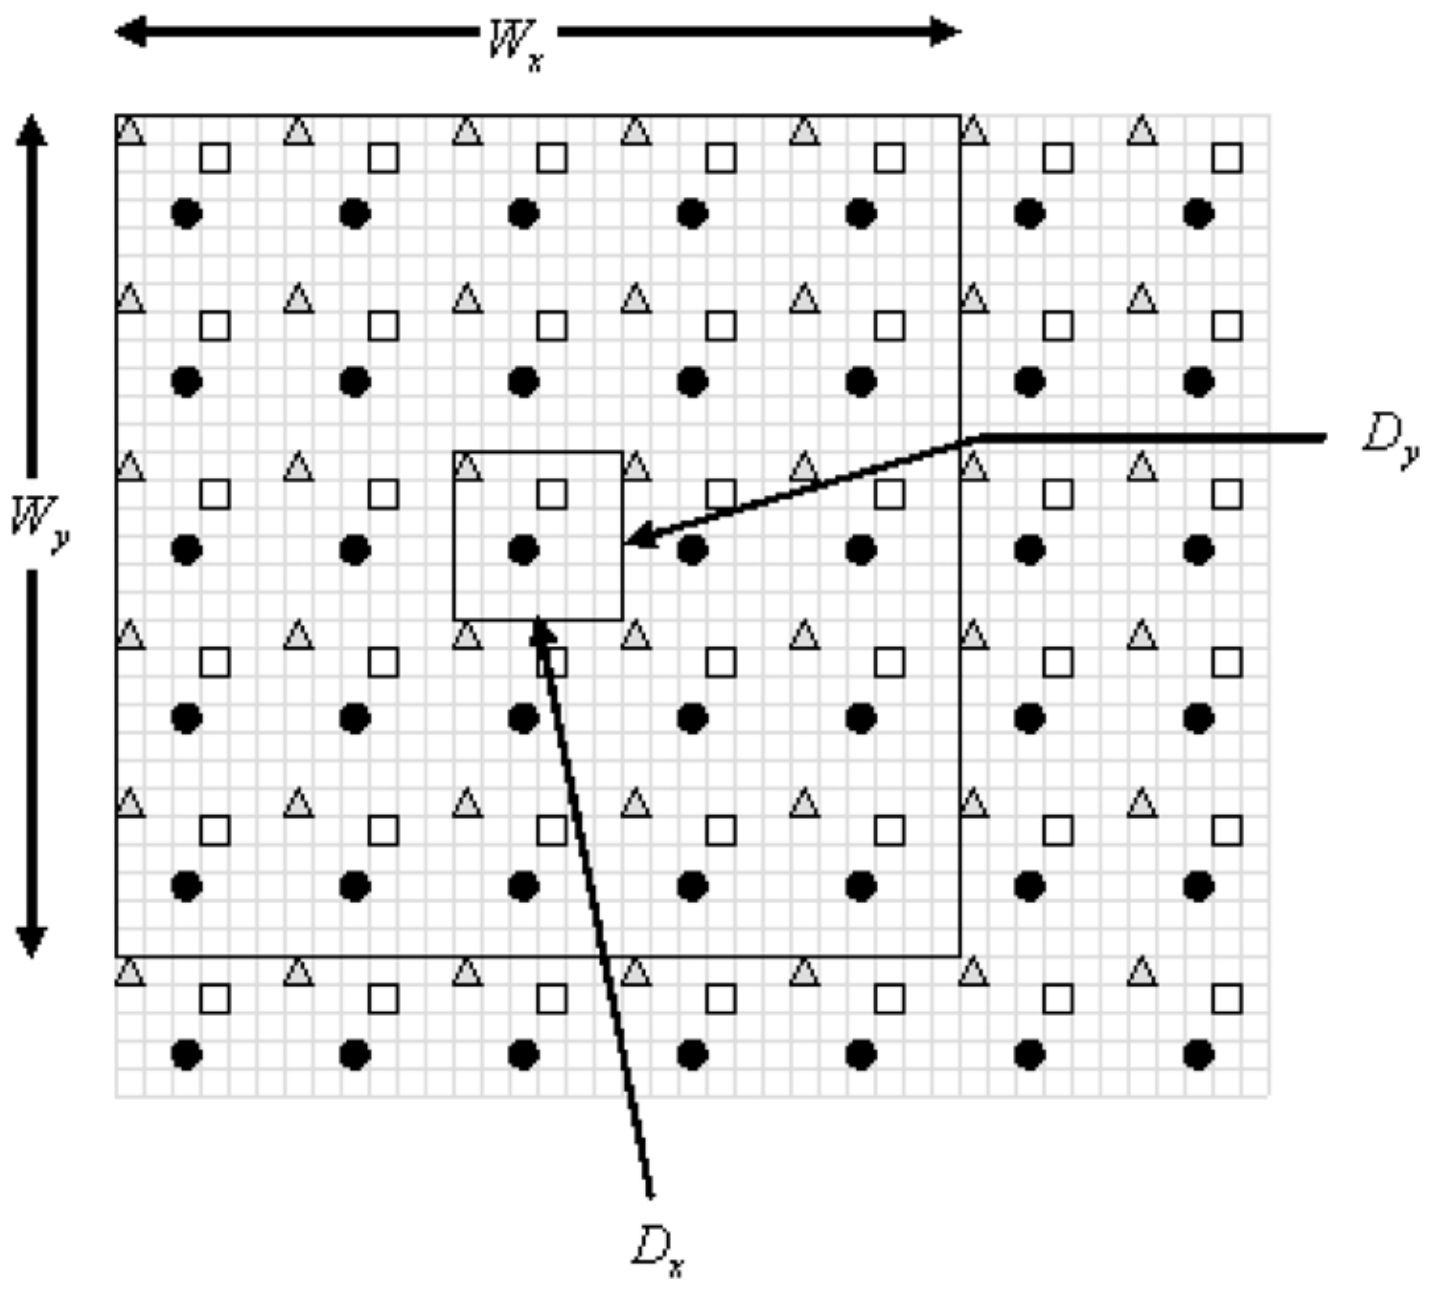
\includegraphics[width=.7\linewidth]{figures/wiener.png}
    \caption{Wiener filter super resolution estimation window of dimension $D_x \times D_y$ and observation window of dimension $W_x \times W_y$\cite{wiener}}
    \label{fig:wiener}
\end{figure}
The pixel values for the estimation window are a function of the wiener filter weights of nearby LR pixels within an observation window whose dimension $W_x, W_y$ are an integer multiple of $D_x, D_y$ (see figure~\ref{fig:wiener}).
%
The weights $\bm{w}$ are defined as the solution to the minimum mean squared error filter problem, i.e. the finite impulse response (FIR) wiener filter:
\begin{equation}
    \bm{w} = R^{-1}\bm{p}
\end{equation}
where $R$ is the auto-correlation of the LR pixels in the observation window and $\bm{p}$ is the cross-correlation between the pixels to be estimated and the LR pixels.
%
$R$ and $\bm{p}$ are both constructed by sampling a parametric model that weights pixels in the observation window according to distance.
%
$R$ is constructed by sampling from
\begin{equation}
    C_1(r) = \sigma_{d}^2 \rho^{r} \ast G(r)
\end{equation}
where $r$ is distance on the HR grid, $\sigma_d$ is related to the empirical variance of all LR pixels in a given observation window and $G(r)$ is a smoothing kernel (e.g. gaussian).
%
Thus by evaluating $C_1$ for all $r = r(n_1, n_2)$ distances between LR pixels $n_1$, $n_2$ we can construct $R$.
%
Similarly $\bm{p}$ is constructed by sampling from
\begin{equation}
    C_2(r) = \sigma_d^2 \rho^{r} \ast G(r) \ast G(-r)
\end{equation}
where here $r = r(m, n)$ is the distance between pixel-to-be-estimated $m$ and LR pixel $n$.
%
Note that $R$ is an $N \times N$ matrix where $N = K W_x W_y/D_x D_y$, i.e. how many LR pixels there are in the observation window, and $\bm{p}$ is an $N \times 1$ column vector uniquely computed for each pixel in the estimation window.
%
The scheme is effective but suffers from issues with the spatial isotropy of the auto-correlation and cross-correlation models.

One the most sophisticated of these non-uniform interpolation schemes employs the kernel regression framework and \textit{steering kernels}\cite{Takeda2007}.
%
In this context we start with all $X_k$ registered to a common HR grid and consider pixel values $Y_i = Y(\bm{x}_i)$ at pixel coordinates $\bm{x}_i = (x_{i1},x_{i2})$ as the measured data pairs $(\bm{x}_i, Y_i)$.
%
Recall that kernel regression frames the estimation problem as
\begin{equation}
    Y_i = Z(\bm{x}_i) + \epsilon
\end{equation}
where $Z$ is the to-be-estimated \textit{regression function} that "predicts" $Y$ as a function of $\bm{x}$.
%
Then $Z$ is assumed to be locally smooth up to some order $N$, i.e. possesses continuous derivatives up to order $N$ and therefore admits an $N$th order Taylor series expansion at some $\bm{x}$ near each of the $\bm{x}_i$
\newcommand*{\bx}{\bm{x}}
\newcommand*{\bxi}{\bm{x}_i}
\newcommand*{\delx}{\bx - \bxi}
\newcommand*{\zbx}{Z(\bx)}
\newcommand*{\zbxi}{Z(\bxi)}
\newcommand*{\bb}{\bm{\beta}}
\newcommand*{\hzbx}{\hat{Z}(\bx)}
\begin{equation}
    \label{eqn:taylor}
    \begin{split}
        \zbxi &= \zbx + \nabla \zbx^T(\delx)\\
        & \quad + \frac{1}{2}(\delx)^T \nabla^2 \zbx (\delx) \\
        & \quad + \cdots + o\left(\left\| \delx \right\|^N \right)
    \end{split}
\end{equation}
where $\nabla Z$ and $\nabla^2 Z$ are the 2-D gradient and Hessian of the regression function.
%
Vectorizing\anote{vectorize} $(\delx)(\delx)^T$, exploiting the symmetry of $\nabla^2 \zbx$, and defining
$\beta_0 = \zbx, \bb_1 = \nabla \zbx$
\begin{align*}
    \bb_2 &= \frac{1}{2}\left[ \frac{\partial^2 \zbx}{\partial x_1^2}, 2 \frac{\partial^2 \zbx}{\partial x_1 \partial x_2}, \frac{\partial^2 \zbx}{\partial x_2^2} \right] \\
\end{align*}
simplifies eqn.~\ref{eqn:taylor} to
\begin{equation}
    \label{eqn:betataylor}
    \begin{split}
        \zbxi &= \beta_0 + \bb_1^T (\delx) \\
        &\quad + \bb_2^T \text{vech}\left( (\delx) (\delx)^T \right) \\
        &\quad + \cdots + o\left(\left\| \delx \right\|^N \right)
    \end{split}
\end{equation}
This suggests using weighted least squares to solve for $\left\{ \bb_n \right\}$ in order to estimate $\hzbx$, i.e.
\begin{equation}
    \hzbx = \min_{\left\{ \bb_n \right\}} \sum_{i=1}^{P} \left[ Y_i - \zbxi \right]^2 K(\delx)
\end{equation}
where $P$ indexes over all pixels in the HR grid and $K$ is \textit{kernel function} whose purpose is to decay the contribution of $\bxi$ if it's in some sense far from $\bx$.
%
In conventional kernel regression $K$ might be any non-negative, symmetric, unimodal\cite{wand1994kernel} function with an additional $H$ parameter that controls the "bandwidth" or "footprint" of the kernel, i.e.
%
\[
    K_H(\delx) = \frac{1}{\det(H)}K\left( H^{-1}(\delx) \right)
\]
with $H = hI$.
\begin{figure}{}
    \centering
    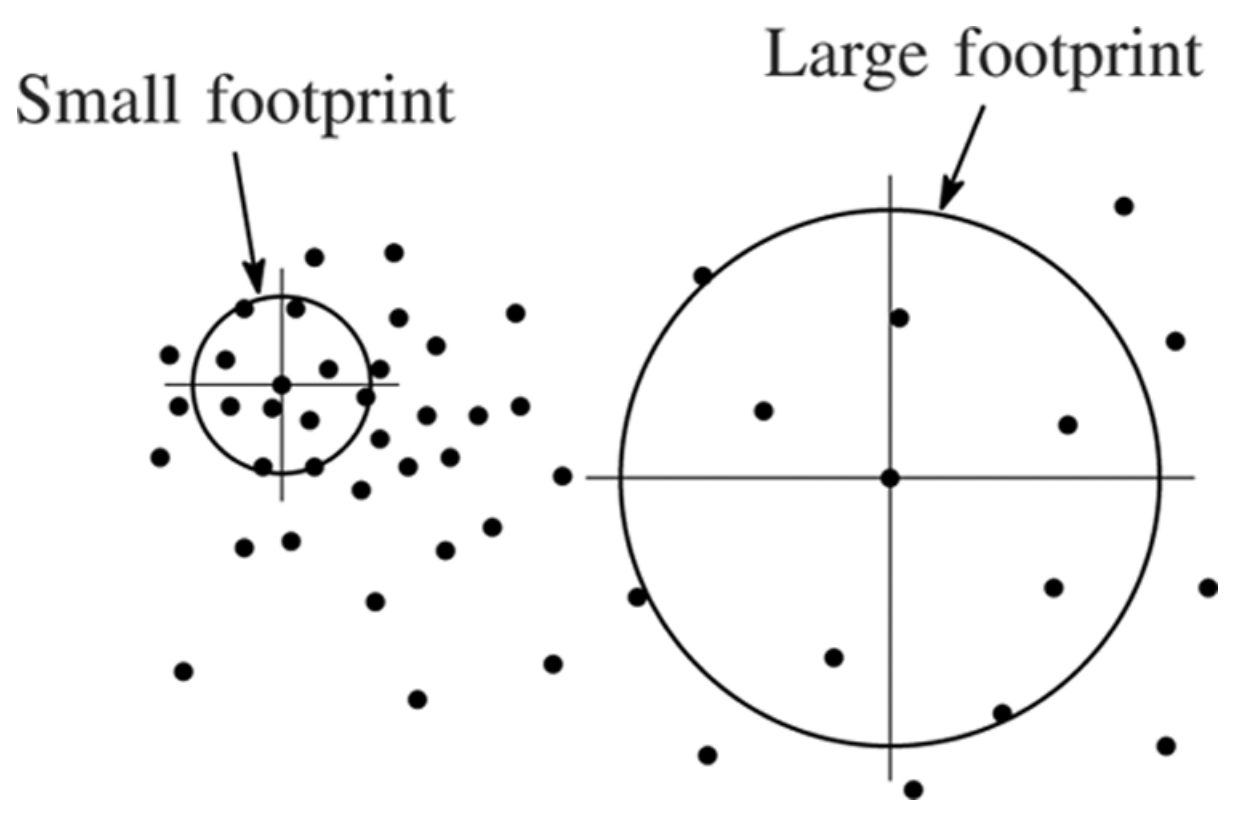
\includegraphics[width=.8\linewidth]{figures/footprint.png}
    \caption{Kernel footprint as a function of sample density\cite{Takeda2007}}
    \label{fig:footprint}
\end{figure}
\begin{figure}{}
    \centering
    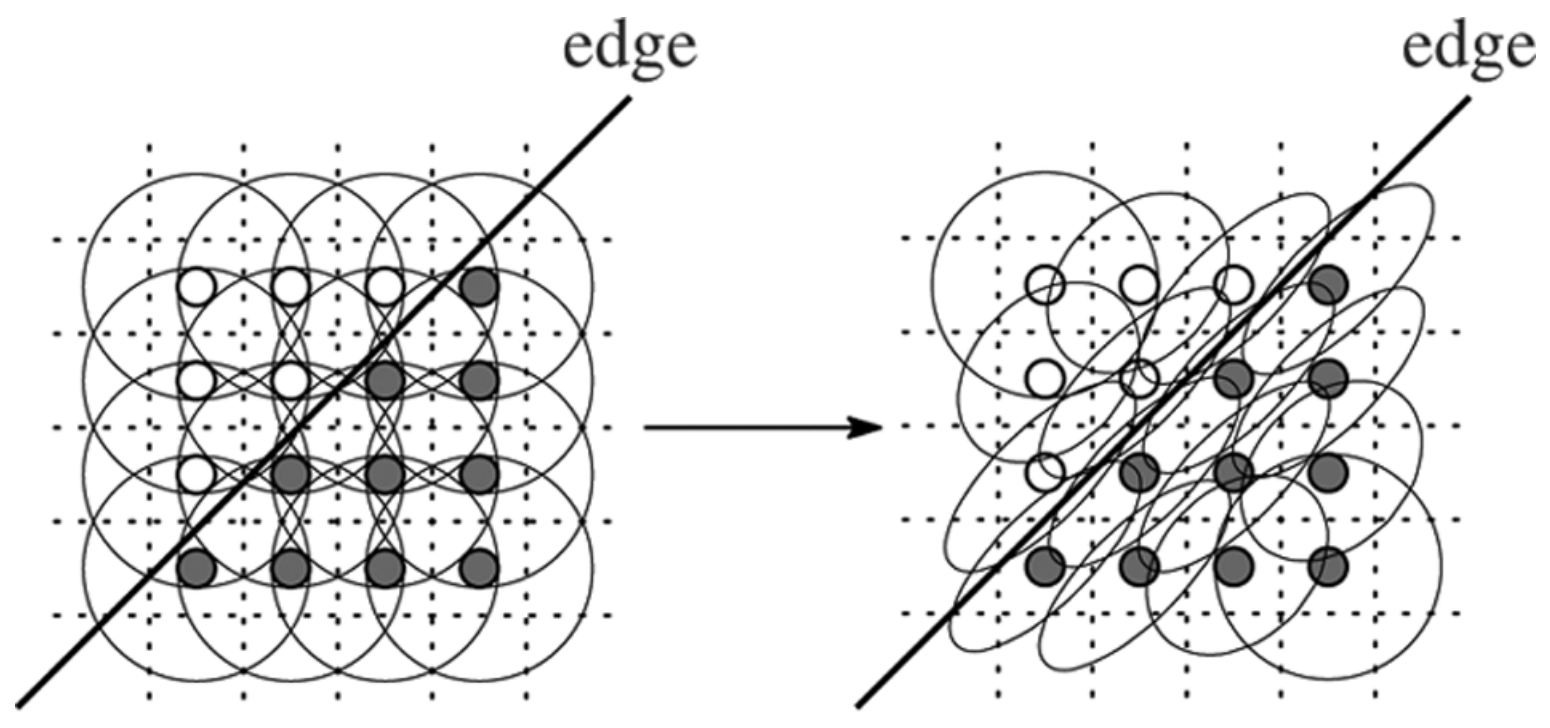
\includegraphics[width=\linewidth]{figures/steering.png}
    \caption{Adapting kernel shape as a function of local directed structure\cite{Takeda2007}}
    \label{fig:steering}
\end{figure}
%
This bandwidth parameter $h$ is useful for enabling kernels to adapt themselves to the local structure of the pixels, e.g. to have larger footprints in sparse sampled regions and have smaller footprints densely sampled regions (see figure~\ref{fig:footprint}).
%
Ultimately though it is desirable to have kernels that can adapt to directed structure in the image, i.e. "steer" the kernel to filter strongly along an edge and weakly across an edge.
%
This is accomplished by, for example, using a Gaussian as the kernel:
\begin{equation}
    K_{H_i}(\delx) \propto \frac{1}{\sqrt{\det{H_i}}}\exp\left\{ -(\delx)^T H^{-1}_i (\delx) \right\}
\end{equation}
and identifying $H_i$ with $\nabla^2 \zbxi$ (since gradients capture edge structure).
%
An estimate $\hat{H}_i$ of $\nabla^2 \zbxi$ can be obtained by looking at covariances of empirical gradients (i.e. the HR grid sampled image convolved with a difference filter).
%
When cast in this light it's obvious that this is essentially a local principal components analysis (PCA) filter.





\subsection{Estimation}
\subsection{Example based}
